\documentclass{beamer}

\usepackage{amssymb,amsmath}
\usepackage{graphicx}
\usepackage{url}
\usepackage{color}
\usepackage{relsize}		% For \smaller
\usepackage{url}			% For \url
\usepackage{epstopdf}	% Included EPS files automatically converted to PDF to include with pdflatex

%For MindMaps
% \usepackage{tikz}%
% \usetikzlibrary{mindmap,trees,arrows}%

%%% Color Definitions %%%%%%%%%%%%%%%%%%%%%%%%%%%%%%%%%%%%%%%%%%%%%%%%%%%%%%%%%
%\definecolor{bordercol}{RGB}{40,40,40}
%\definecolor{headercol1}{RGB}{186,215,230}
%\definecolor{headercol2}{RGB}{80,80,80}
%\definecolor{headerfontcol}{RGB}{0,0,0}
%\definecolor{boxcolor}{RGB}{186,215,230}

%%% Save space in lists. Use this after the opening of the list %%%%%%%%%%%%%%%%
%\newcommand{\compresslist}{
%	\setlength{\itemsep}{1pt}
%	\setlength{\parskip}{0pt}
%	\setlength{\parsep}{0pt}
%}

%\setbeameroption{show notes on top}

% You should run 'pdflatex' TWICE, because of TOC issues.

% Rename this file.  A common temptation for first-time slide makers
% is to name it something like ``my_talk.tex'' or
% ``john_doe_talk.tex'' or even ``discrete_math_seminar_talk.tex''.
% You really won't like any of these titles the second time you give a
% talk.  Try naming your tex file something more descriptive, like
% ``riemann_hypothesis_short_proof_talk.tex''.  Even better (in case
% you recycle 99% of a talk, but still want to change a little, and
% retain copies of each), how about
% ``riemann_hypothesis_short_proof_MIT-Colloquium.2000-01-01.tex''?

\mode<presentation>
{
  % A tip: pick a theme you like first, and THEN modify the color theme, and then add math content.
  % Warsaw is the theme selected by default in Beamer's installation sample files.

  %%%%%%%%%%%%%%%%%%%%%%%%%%%% THEME
  %\usetheme{AnnArbor}
  %\usetheme{Antibes}
  %\usetheme{Bergen}
  %\usetheme{Berkeley}		% bem bacana - menu esquerdo
  %\usetheme{Berlin}
  %\usetheme{Boadilla}
  %\usetheme{boxes}
  %\usetheme{CambridgeUS}		% bem bacana - menu superior
  %\usetheme{Copenhagen}
  %\usetheme{Darmstadt}
  %\usetheme{default}
  %\usetheme{Dresden}
  \usetheme{Frankfurt}
  %\usetheme{Goettingen}
  %\usetheme{Hannover}		% bem bacana - menu esquerdo
  %\usetheme{Ilmenau}
  %\usetheme{JuanLesPins}
  %\usetheme{Luebeck}
  %\usetheme{Madrid}		%bacana
  %\usetheme{Malmoe}
  %\usetheme{Marburg}		% bem bacana - menu direito
  %\usetheme{Montpellier}
  %\usetheme{PaloAlto}		% bem bacana - menu esquerdo
  %\usetheme{Pittsburgh}
  %\usetheme{Rochester}		%bacana
  %\usetheme{Singapore}
  %\usetheme{Szeged}
  %\usetheme{Warsaw}

  %%%%%%%%%%%%%%%%%%%%%%%%%%%% COLOR THEME
  %\usecolortheme{albatross}		% azul escuro, massa
  %\usecolortheme{beetle}		% cinza, menu azul
  %\usecolortheme{crane}		% branco e amarelo, massa
  \usecolortheme{default}		% branco, azul clarinho
  %\usecolortheme{dolphin}		% azul e branco, legal
  %\usecolortheme{dove}			% cinza e branco, feio
  %\usecolortheme{fly}			% todo cinza, horrível
  %\usecolortheme{lily}			% parece o default
  %\usecolortheme{orchid}		% azul e branco, ok
  %\usecolortheme{rose}			% branco e violeta-claro, bonito
  %\usecolortheme{seagull}		% cinza, feio
  %\usecolortheme{seahorse}		% nhé, meio feio
  %\usecolortheme{sidebartab}		% Azul, branco, destaque na tab, interessante
  %\usecolortheme{structure}		% bichado
  %\usecolortheme{whale}		% Azul e branco, bem bonito

  %%%%%%%%%%%%%%%%%%%%%%%%%%%% OUTER THEME
  \useoutertheme{default}
  %\useoutertheme{infolines}
  %\useoutertheme{miniframes}
  %\useoutertheme{shadow}
  %\useoutertheme{sidebar}
  %\useoutertheme{smoothbars}
  %\useoutertheme{smoothtree}
  %\useoutertheme{split}
  %\useoutertheme{tree}

  %%%%%%%%%%%%%%%%%%%%%%%%%%%% INNER THEME
  \useinnertheme{circles}
  %\useinnertheme{default}
  %\useinnertheme{inmargin}
  %\useinnertheme{rectangles}
  %\useinnertheme{rounded}

  %%%%%%%%%%%%%%%%%%%%%%%%%%%%%%%%%%%

  \setbeamercovered{invisible} % or whatever (possibly just delete it)
  % To change behavior of \uncover from graying out to totally
  % invisible, can change \setbeamercovered to invisible instead of
  % transparent. apparently there are also 'dynamic' modes that make
  % the amount of graying depend on how long it'll take until the
  % thing is uncovered.

}


% Get rid of nav bar
\beamertemplatenavigationsymbolsempty

% Use short top
%\usepackage[headheight=12pt,footheight=12pt]{beamerthemeboxes}
%\addheadboxtemplate{\color{black}}{
%\hskip0.5cm
%\color{white}
%\insertshortauthor \ \ \ \ 
%\insertframenumber \ \ \ \ \ \ \ 
%\insertsection \ \ \ \ \ \ \ \ \ \ \ \ \ \ \ \ \  \insertsubsection
%\hskip0.5cm}
%\addheadboxtemplate{\color{black}}{
%\color{white}
%\ \ \ \ 
%\insertsection
%}
%\addheadboxtemplate{\color{black}}{
%\color{white}
%\ \ \ \ 
%\insertsubsection
%}

% Insert frame number at bottom of the page.
% \usefoottemplate{\hfil\tiny{\color{black!90}\insertframenumber}} 

\usepackage[english]{babel}
\usepackage[latin1]{inputenc}
\usepackage{subfigure}

\usepackage{times}
\usepackage[T1]{fontenc}


\title[GB21802]{GB21802 - Programming Challenges}
\subtitle[]{Week 4 - Dynamic Programming (Part II)}
\author[Claus Aranha]{Claus Aranha\\{\footnotesize caranha@cs.tsukuba.ac.jp}}
\institute{College of Information Science}
\date{2015-05-20,23\\{\tiny Last updated \today}}

\begin{document}
%% TODO: Fix makefile so that chapters without TODO do not cause errors.

\section{Introduction}
\subsection{Title}
\begin{frame}
\maketitle
\end{frame}

\subsection{Notes and Warnings}

\begin{frame}
  \frametitle{Last Week Results}
\end{frame}

\begin{frame}
  \frametitle{Special Notes}
\end{frame}

\begin{frame}
  \frametitle{Outline}
  \begin{itemize}
    \item Using DP on the Travelling Salesman Problem
  \end{itemize}
\end{frame}

%%%%%%%%%%%%%%%%%%%%%%%%%%%%%%%%%%%%%%%%
\section{DP for TSP}
\subsection{Traveling Salesman Problems}
\begin{frame}
  \frametitle{Traveling Salesman Problem with DP}

  {\smaller
  \begin{block}{Problem Definition}
    Given $n$ cities and their pairwise distances ($n x n$ dist
    matrix), compute the cost of a \structure{tour} that starts from
    any city $s$, visits all cities \emph{once}, and returns to $s$.
  \end{block}
  \begin{center}
    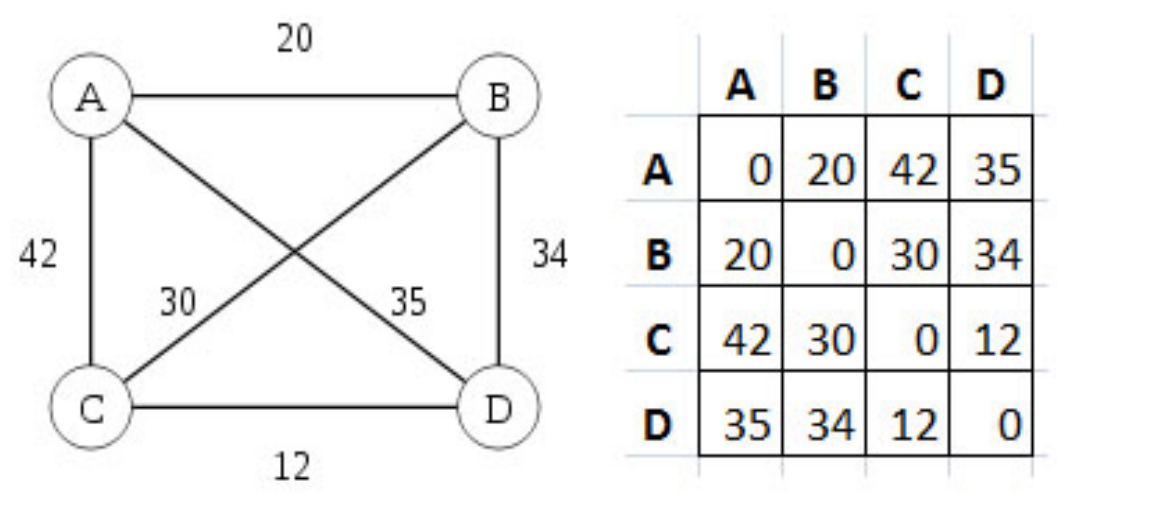
\includegraphics[width=0.7\textwidth]{../img/tsp_example}
  \end{center}

  In the graph above, we have $n=4$ cities and $n! = 24$ possible
  tours (permutations). One minimal tour is A-B-C-D-A, with cost
  $20+30+12+35=97$.
  }
  
  \hrulefill

  \hfill{\tiny Image from Steven Halim -- ``Competitive Programming''}
  
\end{frame}

\begin{frame}[fragile, singleslide]
  \frametitle{TSP -- Complete Search Approach}

  {\smaller 
    A complete search for the TSP tests all city permutations. For each 
    permutation, the complete path of the tour is calculated.
\begin{exampleblock}{}
\begin{verbatim}
#include<algorithm>
int c[4] = {0,1,2,3};
do {
  cost = 0;
  for (i=0;i<4;i++)
    cost += pathcost[c[i]][c[(i+1)%4];
} while (next_permutation(c,c+4));
\end{verbatim}
\end{exampleblock}

  \begin{block}{Overlapping subproblems}
    Complete search costs $O(n!n)$, so the biggest $n$ we can
    realistically handle on a programming competition is \structure{10
      or 11.}
    
    \medskip

    However, many subpaths in the tour are repeated. For example:
    \begin{itemize}
    \item A-B-(n-2)
    \item B-A-(n-2)
    \end{itemize}
    Have $(n-2)!$ repeated subproblems. A DP approach should be possible!    
  \end{block}
  }
  
\end{frame}

\begin{frame}
  \frametitle{TSP -- DP Approach}
  {\smaller
  \begin{block}{Basic Recurrence}
    \begin{itemize}
    \item If all cities are visited, return the cost from the last
      city to the first one.
    \item If not all cities are visited, try each unvisited city and
      select the one with the minimum cost.
    \end{itemize}
  \end{block}

  \begin{block}{State Table}

    Note that this recurrence requires \structure{the set of cities
      already visited} and \structure{the city currently being
      visited}.


    \bigskip

    This means that our state is \emph{(visitset,city)}. Our table has
    size $2^nn$, and each state can be calculated in time $O(n)$, so
    our DP-TSP has complexity $O(n^22^n)$. 

    \bigskip
    
    Not a huge improvement, but now we can solve problems up to size
    $n \leq 16$.

  \end{block}}
\end{frame}

\begin{frame}[fragile,singleslide]
  \frametitle{TSP -- DP Code}

{\smaller
  \begin{exampleblock}{}
\begin{verbatim}
int dp[n][1<<n] = -1
start = 0

visit(p,v):
   if (v == (1<<n) - 1):
      return cost[p][start]
   if dp[p][v] != -1
      return dp[p][v]

   tmp = MAXINT
   for i in n:
       if not(v && (1 << i):
           tmp = min(tmp,
                     cost[p][i] + visit(i, v | (1<<i)))

   dp[p][v] = tmp
   return tmp

\end{verbatim}
  \end{exampleblock}}
\end{frame}

%%%%%%%%%%%%%%%%%%%%%%%%%%%%%%%%%%%%%%%%%%%%%%%%%%%%%%%%%%%%%%%%%%%%%%
\section{Other DP}

\subsection{UVA 10943 -- How do you add?}
\begin{frame}
  \frametitle{UVA 10943 -- How do you add?}
  \begin{block}{Problem Description}
    Given an integer $n$, how many ways can you add $K$ integers ($0 \leq
    i \leq n$) so that their sum is equal to $n$?
 
    \bigskip

    Example: $n = 20, K = 2$\\
    $0 + 20, 1 + 19, 2 + 18, \ldots, 20+0$ 
  \end{block}

  What is the recurrence?

  \begin{itemize}
  \item When K = 1, there is only one way to add to n.
  \item When K = i > 1, we can test all numbers X between 0 and n, and
    our result will be the sum of all $(n-X,K-1)$ sub problems.\\
  \end{itemize}
\end{frame}

\begin{frame}
  \frametitle{How do you add? -- Recurrence Example}

  Recurrence Example: $n = 10, K = 3$

  \bigskip

  {\smaller

    \begin{tabular}{rl}
      ways(10,3) = & (0,ways(10,2)) + \\
      & (1,ways(9,2)) + \\
      & (2,ways(8,2)) + \\
      & ...\\
      & (10,ways(0,2))\\
      \hline
      ways(8,2) = & (0,ways(8,1)) + \\
      & (1,ways(7,1)) + \\
      & ...\\
      & (8,ways(0,1))\\
      = & 9\\ 
      \hline
      ways (10,3) = &$11 + 10 + 9 + 8 + \ldots + 1 = 66$ \\
    \end{tabular}
  }

\end{frame}

\begin{frame}[fragile,singleslide]
  \frametitle{How do you add? -- Bottom-Up DP}

{\smaller
\begin{exampleblock}{}
\begin{verbatim}
dp[maxK][maxN]
tsum[2][maxN]

for (i in maxN):
   tsum[1][i] = i+1
   dp[1][i] = 1

for (i in K):
   tsum[0] = tsum[1]
   for (j in maxN):
      dp[i][j] = tsum[0][j]
      tsum[1][j] = tsum[1][j-1] + tsum[0][j]
\end{verbatim}
\end{exampleblock}}

\bigskip

Time complexity is $O(nK)$
\end{frame}

\begin{frame}
  \frametitle{How do you Add? -- Mathematical Approach} 

  This problem can also be seen as solving the recurrence/closed form
  of a binomial combination C. We will come back to recurrences in a
  later class.
\end{frame}

\subsection{DP Ideas}
\begin{frame}
  \frametitle{Thinking About DP -- 1} 
  {\small 

    DP can come in many forms other than its classical problems. You
    can solve these problems following the procedure that we have seen
    so far:
    \begin{enumerate}
    \item Elaborate a recursive, full search solution.
    \item Define the \structure{distinct states} and the
      \structure{transitions}
    \item Write a program for \structure{memoizing} the state table
      (top-down) or \structure{constructing} the table (bottom up).
    \end{enumerate}

    \bigskip

    \begin{block}{}
      DP has an intrinsic relationship with \alert{Directed Acyclic
        Graph (DAG)}. States are mapped to vertexes, transitions to
      edges. We will explore this relationship more in the future.
      %% TODO: Explore this relationship more in the future
    \end{block}
  }
\end{frame}

\begin{frame}
  \frametitle{Thinking About DP -- 2}
  {\smaller
  Common ways to imagine DP states:
  \begin{block}{Position in the problem state}
    \begin{itemize}
    \item The original problem is an array of values: $\{x_1,x_2,\ldots,x_n\}$
      \medskip

    \item Subproblems based on position in the array:\\
      \structure{Suffix}: $\{x_1, x_2,\ldots,x_{n-1}\} + x_n$\\
      \structure{Prefix}: $x_1 + \{x_2,x_3,\ldots,x_n\}$\\
      \structure{Two sub-problems}: $\{x_1,x_2,\ldots,x_i\}+\{x_{i+1},x_{i+2},\ldots,x_n\}$
      \medskip

    \item Can be generalized for 2D (x,y): Consider the size of the table!
    \end{itemize}
  \end{block}
  }
\end{frame}

\subsection{UVA 10003 -- Cutting Sticks}
\begin{frame}
  \frametitle{UVA 10003 -- Cutting Sticks}
  
  {\smaller
  \begin{block}{Problem Description}
    Given a stick of length $1 \leq l \leq 1000$ and $1 \leq n \leq
    50$ cuts (positions) to be made, the cost of a cut is given by the length of 
    the stick being cut.

    \medskip

    Find a cutting sequence that minimizes the cost of cutting the stick.
  \end{block}
  
  \medskip

  \structure{Example:} $l=100, n=3, cuts=\{25,50,75\}$

  \begin{center}
    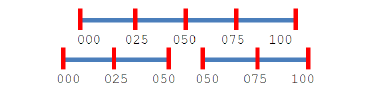
\includegraphics[width=0.6\textwidth]{../img/cuttingsticks}
  \end{center}

  \begin{itemize}
  \item Sequence 1: 25, 50, 75. Cost: 100 + 75 + 50 = 225
  \item Sequence 2: 50, 25, 75. Cost: 100 + 50 + 50 = 200
  \end{itemize}

  \begin{block}{}
  What is the recurrence to find the minimum cost?
  \end{block}
  }
\end{frame}

\begin{frame}
  \frametitle{Cutting Sticks -- Recurrence}
  {\smaller
    \structure{Basic Idea}: Price(start,end) = end-start + Price(start,cut) + Price(cut,end)

    \medskip

    \alert{Problem}: Using start/end, we have 1000*1000 states.

    \medskip
    
    \structure{Solution}: We use cut indexes instead! (50*50 states)

    \vfill

    \begin{block}{Recurrence using cut index:}
    \begin{itemize}
    \item Price(i,i+1) = 0 
    \item Price(i,j) = min(Size[j] - Size[i] + Price(i,k) + Price(k,j))\\
      (for all $i < k < j$)        
    \end{itemize}
    \end{block}


    \medskip
    
    Note that the recurrence costs $O(n)$, and the table size is $O(n^2)$, 
    so the total cost is $O(n^3)$ }
\end{frame}


\section{More Examples}
\subsection{DP on Math Problems}

\begin{frame}
  \frametitle{DP on Math Problems}
  Many math problems can be implemented as DP:
  \begin{itemize}
  \item Combinatoric problems often have recursive formulas, and
    overlapping subproblems;
    \begin{itemize}
    \item Fibonacci Number: $f(n) = f(n-1)+f(n-2)$
    \end{itemize}
  \item Probability problems often require you to search the entire
    probability space (tree). These trees usually have overlapping branches.
  \item Maths problems on static data (sum, min, max)
  \end{itemize}
\end{frame}

% TODO: Add a DP math example (Yahtzee?)
%\begin{frame}
%  \frametitle{DP on Math Problems}
%\end{frame}


\begin{frame}
  \frametitle{DP on Strings}
  \begin{itemize}
  \item edit distance, substring manipulation, etc.
  \item Usually, we don't send the string in the recurrence, but
    \structure{indexes on the string}\\
    %% TODO: Add an string problem
  \end{itemize}
\end{frame}

\begin{frame}
  \frametitle{DP Issues}
  
  {\small
  \begin{itemize}
  \item Many DP problems look like ``non DP'' problems. 

    \begin{block}{Example}
      Select positions for a set of flags that cover a certain
      radius, in order to maximize area coverage. 

      \medskip
      
      The area calculation requires geometry, but the flag selection is 
      usually DP.
    \end{block}
    
    \medskip
    
  \item Some problem have sub-problems, but they are not overlapping.\\
    (In this case, DP will not work, but maybe Divide and Conquer?)
  \end{itemize}}
\end{frame}

\subsection{A few more problems}
% Add discussion for a few more problems


\section{Conclusion}
\subsection{Conclusion}
\begin{frame}
  \frametitle{That's all for DP!}
  This is what we've seen for weeks 3 and 4:

  \begin{itemize}
  \item DP = Complete Search + State table;
  \item Good when many \structure{overlapping subproblems} exist;
  \item Top-Down (recursive) and Bottom-Up (nested loops);
  \item Classical DP problems;
  \item (some!) non-classical DP problems;
  \end{itemize}

  \vfill

  For the next two weeks, the theme will be \structure{graph algorithms}!
\end{frame}

\subsection{Week 4 Problems}
\begin{frame}
  \frametitle{Problems for Week 4}
  \begin{itemize}
  \item Collecting Beepers
  \item Shopping Trip
  \item Bar Codes
  \item Cutting Sticks
  \item String Popping
  \item Divisibility
  \item Marks Distribution
  \item Squares
  \end{itemize}

\end{frame}

\begin{frame}
  \frametitle{World Finals Problem - 2016 Problem C}
  {\smaller
  \begin{block}{Problem Description -- Ceiling Function}
    Given $n$ arrays with $K$ values each, each array 
    is organized in a binary search tree in the order of input. 

    \bigskip
    
    In other words, the first element is the root, the second
    is the left child of the root if smaller, right child if bigger, 
    so on.

    \bigskip

    Count the number of different trees generated by the input data.    
  \end{block}

  \begin{center}
    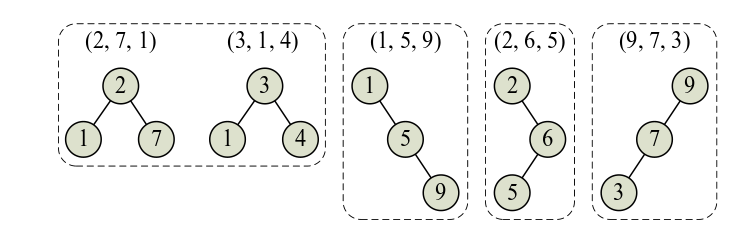
\includegraphics[width=0.7\textwidth]{../img/worldfinal2016}
  \end{center}

  }
\end{frame}


\end{document}



